\emph{This chapter gives a general overview of hydraulic systems and an introduction to the WSS in Randers. The basic topology and structures of water supply networks are explained. Furthermore, the basic components of hydraulic systems are discussed and the unit called head, as an alternative measure of pressure, is introduced.}

\section{Hydraulic system overview}
\label{hydraulic_system_overview}

WSSs are designed to deliver water to consumers in terms of sufficient pressure and appropriate chemical composition. Distribution systems as such are typically transport water from one geographical place to another. In practice, there are different methods existing to achieve this water transport. One example is to make use of natural advantages such as the water stored in mountains, and thereby use the potential energy of the water to provide pressure in the network. Examples for this are countries like Norway and Sweden where the advantages of the landscape are being exploited. However, in this project the source of the water is considered as groundwater, considering that in Denmark all reservoirs in the network are tapping water from the ground. After tapping the water, it goes through a cleaning process at the waterworks and afterwards the pure water is pumped into the network \cite{prahata}. In WSSs, pumps and valves are the elements that enable the delivery of water to the consumers or to elevated reservoirs, storing water for later use. Such a network is illustrated in the figure below: 

%illustration of WSS
\begin{figure}[H]
\centering

\includegraphics[width=0.35\textwidth]{report/pictures/missingfigure}
\caption{Illustration of a WSS.}
\label{fig:WSS_example}
\end{figure}

The delivered water needs to fulfil a certain pressure criteria in order to reach consumers at higher levels. For example, in some cases the pressure has to be high enough to make it to the fourth floor of a building and still provide appropriate pressure in the water taps. Generally, in such cases booster pumps are placed in the area, helping to supply the pressure. Too large pressure values, however increase water losses due to pipe waste \cite{walski2003advanced}.

Another criteria is that the flow through particular pipes need to stay within acceptable limits. A low flow rate can lead to water quality problems due to the undesirable microorganisms in the water and due to the metal and salt accumulation on the wall of the pipes \cite{walski2003advanced}. 

As can be seen in \figref{fig:WSS_example}, typically WSSs consist of pipe, valve, reservoir, elevated reservoir(tank) and pump components. The common property of them is that they are all two-terminal components, therefore they can be characterized by the dynamic relationship between the pressure drop across their two corresponding endpoints and the flow through them \cite{master_aau}. 

\subsection{Pipe networks}
\label{pipe_networks}

Pipes are the most common components of WSSs since they are used for carrying pressurized water. They serve as a connection between components. Normally, the pipe network can be split into different sub-parts, taking into account the physical characteristics and the attributes of the pipes. Therefore, water supply networks can consist of transmission mains, arterial mains, distribution mains and service lines as shown in the example below: 

%illustration of pipe topology / loop configuration
\begin{figure}[H]
\centering
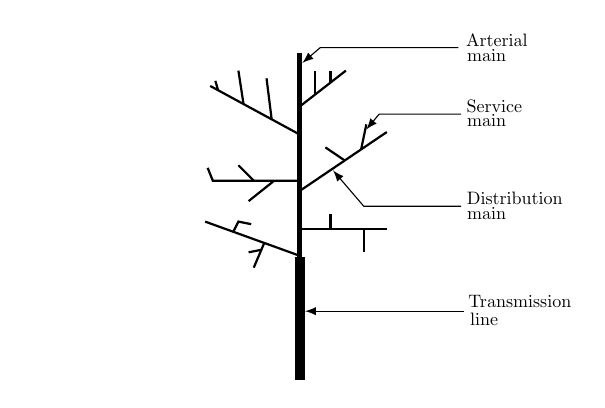
\begin{tikzpicture}[scale=0.65,transform shape]

\fill [black] (0.1,0.1) rectangle (0.3,2.5);
\fill [black] (0.15,6.5) rectangle (0.25,2.5);

\draw [thick](0.15,2.55) -- (-1.65,3.2);
\draw [thick](-0.5,2.77) -- (-0.7,2.3);
\draw [thick](-0.55,2.65) -- (-0.8,2.6);
\draw [thick](-1.1,3) -- (-1,3.2) -- (-0.75,3.15);
\draw [thick](0.2,3.05) -- (1.9,3.05);
\draw [thick](0.8,3.05) -- (0.8,3.35);
\draw [thick](1.45,3.05) -- (1.45,2.6);
\draw [thick](0.2,4) -- (-1.5,4) -- (-1.6,4.25);
\draw [thick](-0.3,4) node (v1) {} -- (-0.8,3.6);
\draw [thick](v1);
\draw [thick](-0.7,4) -- (-1,4.3);
\draw [thick](0.2,3.8) -- (1.9,4.95);
\draw [thick](1.4,4.62) -- (1.5,5.1);
\draw [thick](1.07,4.4) -- (0.7,4.65);
\draw [thick](0.2,4.9) -- (-1.55,5.85);
\draw [thick](-0.35,5.2) -- (-0.45,6);
\draw [thick](-0.9,5.5) -- (-1,6.15);
\draw [thick](-1.4,5.78) -- (-1.45,5.95);
\draw [thick](0.2,5.45) -- (1.1,6.15);
\draw [thick](0.8,5.92) -- (0.8,6.15);
\draw [thick](0.5,5.69) -- (0.5,6.15);
%\draw [-latex](3.4,1.45) -- (0.3,1.85);
\node at (4.5,1.65) {\normalsize Transmission};
\node at (3.8,1.3) {\normalsize line};
%\draw [-latex](3.35,3.4) -- (0.6,4.05);
\node at (4.4,3.65) {\normalsize Distribution};
\node at (3.85,3.35) {\normalsize main};
\node at (4,5.45) {\normalsize Service};
\node at (3.85,5.17) {\normalsize main};
\node at (4.05,6.75) {\normalsize Arterial};
\node at (3.85,6.45) {\normalsize main};
%\draw [-latex](3.25,5.25) -- (1.5,5);
%\draw [-latex](3.2,6.55) -- (0.25,6.4);
\node at (-5,3.6) {         };
\draw [-latex](3.3,6.6) -- (0.6,6.6) -- (0.25,6.3);
\draw [-latex](3.35,5.3) -- (1.75,5.3) -- (1.5,5);
\draw [-latex](3.35,3.5) -- (1.45,3.5) -- (0.85,4.2);
\draw [-latex](3.4,1.45) -- (0.3,1.45);
\end{tikzpicture} 
\caption{Illustration of pipe mains. Tree configuration.}
\label{fig:pipemain_example}
\end{figure}

Transmission mains deliver large amounts of water over long distances. Arterial and distribution mains provide intermediate steps towards delivering water to the end-users. Service lines transmit the water from the distribution mains straight to the end-users \cite{grigg2012water}.

The transmission and distribution network can have a topology that is called a loop or a tree structure. \figref{fig:pipemain_example} shows an example for a tree configuration. This type of configuration is most frequently used in rural areas \cite{mays}. Typically the network has only one path for the water to reach the end-users. Common problems with this configuration is that on the outer parts of the system lower pressures can be experienced due to the pressure losses from long flow paths. The flow dynamics within this kind of systems therefore consist of large flows closer to the source that turn into smaller flows on the outer parts of the system. Main disadvantage of a purely tree structure system is that due to maintenance or momentary breakdowns, the system suffers disruption of service \cite{mays}. 

Loop networks have a configuration as shown in \figref{fig:loop_configuration}. 

%illustration of loop configuration
\begin{figure}[H]
\centering
 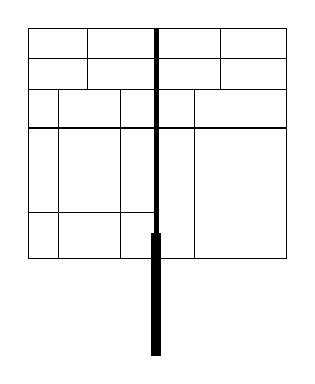
\begin{tikzpicture}[scale=0.65,transform shape]
 
 
\fill [black] (0.1,0.1) rectangle (0.3,2.5);
\fill [black] (0.15,6.5) rectangle (0.25,2.5);


%\node at (-6,3.6) {         };

\draw (0.2,6.5) -- (2.75,6.5) -- (2.75,2) -- (0.3,2);
\draw (0.2,6.5) -- (-2.3,6.5) -- (-2.3,2) -- (0.1,2);
\draw (-2.3,5.3) -- (2.75,5.3);
\draw (-2.3,5.9) -- (2.75,5.9);
\draw (-1.15,6.5) -- (-1.15,5.3);
\draw (1.45,6.5) -- (1.45,5.3);
\draw (-1.7,5.3) -- (-1.7,2);
\draw (-0.5,5.3) -- (-0.5,2);
\draw (-2.3,4.55) -- (0.15,4.55);
\draw (-2.3,2.9) -- (0.15,2.9);
\draw (0.95,5.3) -- (0.95,2);
\draw (0.2,4.55) -- (2.75,4.55);
\end{tikzpicture} 
%
\includegraphics[width=0.35\textwidth]{report/pictures/missingfigure}
\caption{Loop configuration.}
\label{fig:loop_configuration}
\end{figure}

Loop networks are usually composed of smaller loops which made up of smaller distribution mains, and larger loops that are connected to arterial or transmission mains. Elevated reservoirs are typically placed in the centre of the system due to pressure losses resulting from flows through the loop network \cite{council2007drinking}. In the presence of the larger loops, they may be used to feed an internal distribution grid or a distribution grid attached to the outer part of the loop. Loop configurations are generally associated with larger suburban and city distribution systems such as the WSS in Randers\cite{council2007drinking}. 

\subsection{Elevated reservoirs}
\label{elevated_reservoirs}

Elevated reservoirs, or tanks, are typically placed in the system to use them as buffers and level out the pressure and flow demand differences. When the demand is high, the waterworks might not be able to provide the sufficient amount of water in the network. In these cases, the elevated reservoir supplies the remaining demand. When the user consumption decreases, the system can be controlled such that the tank is being refilled to provide the required demand for the next peak time of consumption. Having such an elevated reservoir in the network, the system becomes more independent of the pump stations, as the refilled tank can itself maintain the desired pressure and flow for a limited time. 

Due to the elevation of the tank, when it is filled up, the pumping stations need to provide a pressure higher than the pressure in the water tank. Therefore when the tank is being emptied, the pumping stations can reduce the amount of pressure they provide to the system, since the pressure from the elevated reservoir becomes dominant. This is due to that the dynamics of systems with large storages come primarily from the pressure of the tank \cite{8thsemester_project}. This is due to the height change of the tank being very slow because of the large diameter of the tank. Due to these considerations, the effect of these elevated reservoirs has to be taken into account while modelling the system. 

\subsection{Pumps}
\label{pumps}

Water pumps are used to increase pressure in hydraulic systems, thus making the water flow. Pumps are typically the main actuators of a WSS and they can be either flow or pressure controlled. Therefore, pumps can have controllers to produce a desired flow or pressure. This is done by changing the rotational speed of the pump. In this way, when the pump has a reference pressure or flow, simple control makes it possible to produce the desired flow or pressure respectively \cite{kallesoePHD}.The pressure required to make the water reach some height is the sum of the pressure required to overcome the elevation and the friction losses in the pipe network. 

The most common pumps in WSSs are centrifugal pumps. Normally, the characteristics of such pumps are described by two pump curves. The two curves depict the volume flow versus the pressure and the power of the pump respectively. Normally the curves describe the characteristics for one particular speed, which is denoted the nominal speed \cite{kallesoePHD}. An example of these pump curves is shown in \figref{fig:pump_curves}.

\begin{figure}[H]
\centering
\begin{subfigure}{.49\textwidth}
\centering
  % This file was created by matlab2tikz.
%
%The latest updates can be retrieved from
%  http://www.mathworks.com/matlabcentral/fileexchange/22022-matlab2tikz-matlab2tikz
%where you can also make suggestions and rate matlab2tikz.
%
\definecolor{mycolor1}{rgb}{0.00000,0.44700,0.74100}%
%
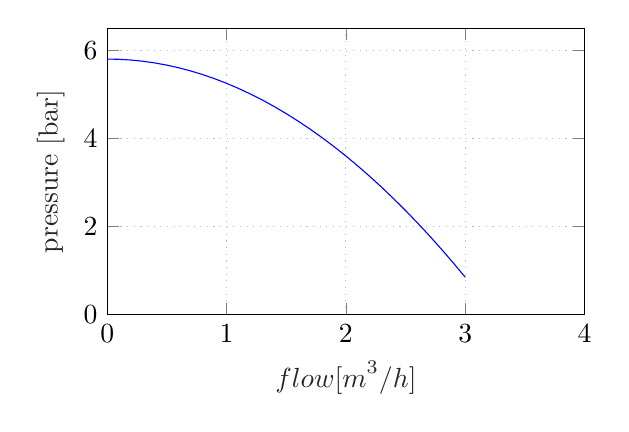
\begin{tikzpicture}

\begin{axis}[%
width=0.5\textwidth,
height=0.3\textwidth,
at={(0.758in,0.499in)},
scale only axis,
xmin=0,
xmax=4,
xlabel style={font=\color{white!15!black}},
xlabel={$\text{flow [m}^\text{3}\text{/h]}$},
ymin=0,
ymax=6.5,
ylabel style={font=\color{white!15!black}},
ylabel={pressure [bar]},
axis background/.style={fill=white},
xmajorgrids,
ymajorgrids,
grid style={dotted}
]
\addplot [color=blue, forget plot]
  table[row sep=crcr]{%
0	5.8\\
0.0999999999999996	5.7945\\
0.2	5.778\\
0.3	5.7505\\
0.4	5.712\\
0.5	5.6625\\
0.600000000000001	5.602\\
0.7	5.5305\\
0.8	5.448\\
0.9	5.3545\\
1	5.25\\
1.1	5.1345\\
1.2	5.008\\
1.3	4.8705\\
1.4	4.722\\
1.5	4.5625\\
1.6	4.392\\
1.7	4.2105\\
1.8	4.018\\
1.9	3.8145\\
2	3.6\\
2.1	3.3745\\
2.2	3.138\\
2.3	2.8905\\
2.4	2.632\\
2.5	2.3625\\
2.6	2.082\\
2.7	1.7905\\
2.8	1.488\\
2.9	1.1745\\
3	0.85\\
};
\end{axis}
\end{tikzpicture}% 
  \caption{Flow versus pressure difference}
  \label{fig:sub1}
\end{subfigure}
\begin{subfigure}{.49\textwidth}
\centering
  % This file was created by matlab2tikz.
%
%The latest updates can be retrieved from
%  http://www.mathworks.com/matlabcentral/fileexchange/22022-matlab2tikz-matlab2tikz
%where you can also make suggestions and rate matlab2tikz.
%
\definecolor{mycolor1}{rgb}{0.00000,0.44700,0.74100}%
%
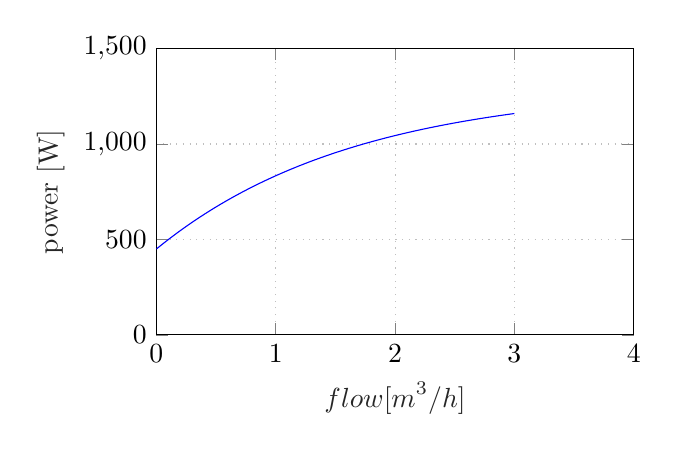
\begin{tikzpicture}

\begin{axis}[%
width=0.5\textwidth,
height=0.3\textwidth,
at={(0.758in,0.499in)},
scale only axis,
xmin=0,
xmax=4,
xlabel style={font=\color{white!15!black}},
xlabel={$\text{flow [m}^\text{3}\text{/h]}$},
ymin=0,
ymax=1500,
ylabel style={font=\color{white!15!black}},
ylabel={power [W]},
axis background/.style={fill=white},
xmajorgrids,
ymajorgrids,
grid style={dotted}
]
\addplot [color=blue, forget plot]
  table[row sep=crcr]{%
0	450\\
0.0599999999999454	480.055750539345\\
0.119999999999891	509.048738560475\\
0.180000000000064	537.01654303413\\
0.240000000000009	563.995414149676\\
0.299999999999955	590.020320300419\\
0.3599999999999	615.124993407542\\
0.420000000000073	639.341972641396\\
0.480000000000018	662.702646596815\\
0.539999999999964	685.237293977134\\
0.599999999999909	706.975122839624\\
0.660000000000082	727.944308453222\\
0.720000000000027	748.172029817625\\
0.779999999999973	767.684504891077\\
0.839999999999918	786.507024572515\\
0.900000000000091	804.663985482109\\
0.960000000000036	822.178921582701\\
1.01999999999998	839.074534683114\\
1.07999999999993	855.372723862874\\
1.1400000000001	871.094613856482\\
1.20000000000005	886.260582434024\\
1.25999999999999	900.890286813621\\
1.31999999999994	915.002689139926\\
1.38000000000011	928.616081061725\\
1.44000000000005	941.74810744047\\
1.5	954.415789220491\\
1.55999999999995	966.635545490521\\
1.61999999999989	978.423214765135\\
1.68000000000006	989.79407551368\\
1.74000000000001	1000.76286596331\\
1.79999999999995	1011.3438032018\\
1.8599999999999	1021.55060160486\\
1.92000000000007	1031.39649061192\\
1.98000000000002	1040.89423187328\\
2.03999999999996	1050.05613579107\\
2.09999999999991	1058.8940774752\\
2.16000000000008	1067.41951213515\\
2.22000000000003	1075.64348992761\\
2.27999999999997	1083.57667027892\\
2.33999999999992	1091.22933570126\\
2.40000000000009	1098.6114051202\\
2.46000000000004	1105.73244673099\\
2.51999999999998	1112.60169040034\\
2.57999999999993	1119.22803962954\\
2.6400000000001	1125.62008309472\\
2.70000000000005	1131.78610577893\\
2.75999999999999	1137.73409971065\\
2.81999999999994	1143.47177432257\\
2.88000000000011	1149.00656644414\\
2.94000000000005	1154.34564994065\\
3	1159.49594501165\\
};
\end{axis}
\end{tikzpicture}% 
  \caption{Flow versus power consumption}
  \label{fig:sub2}
\end{subfigure}
\caption{Pump curves describing the performance of a centrifugal pump at nominal speed.}
\label{fig:pump_curves}
\end{figure}

% %pump curves
% \begin{figure}[H]
% \centering
% % This file was created by matlab2tikz.
%
%The latest updates can be retrieved from
%  http://www.mathworks.com/matlabcentral/fileexchange/22022-matlab2tikz-matlab2tikz
%where you can also make suggestions and rate matlab2tikz.
%
\definecolor{mycolor1}{rgb}{0.00000,0.44700,0.74100}%
%
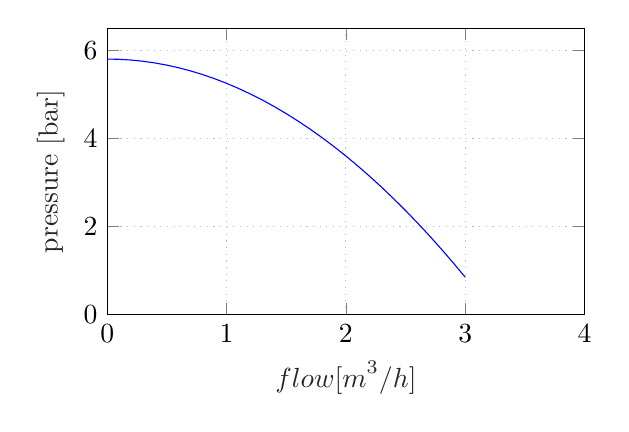
\begin{tikzpicture}

\begin{axis}[%
width=0.5\textwidth,
height=0.3\textwidth,
at={(0.758in,0.499in)},
scale only axis,
xmin=0,
xmax=4,
xlabel style={font=\color{white!15!black}},
xlabel={$\text{flow [m}^\text{3}\text{/h]}$},
ymin=0,
ymax=6.5,
ylabel style={font=\color{white!15!black}},
ylabel={pressure [bar]},
axis background/.style={fill=white},
xmajorgrids,
ymajorgrids,
grid style={dotted}
]
\addplot [color=blue, forget plot]
  table[row sep=crcr]{%
0	5.8\\
0.0999999999999996	5.7945\\
0.2	5.778\\
0.3	5.7505\\
0.4	5.712\\
0.5	5.6625\\
0.600000000000001	5.602\\
0.7	5.5305\\
0.8	5.448\\
0.9	5.3545\\
1	5.25\\
1.1	5.1345\\
1.2	5.008\\
1.3	4.8705\\
1.4	4.722\\
1.5	4.5625\\
1.6	4.392\\
1.7	4.2105\\
1.8	4.018\\
1.9	3.8145\\
2	3.6\\
2.1	3.3745\\
2.2	3.138\\
2.3	2.8905\\
2.4	2.632\\
2.5	2.3625\\
2.6	2.082\\
2.7	1.7905\\
2.8	1.488\\
2.9	1.1745\\
3	0.85\\
};
\end{axis}
\end{tikzpicture}% 
% %
\includegraphics[width=0.35\textwidth]{report/pictures/missingfigure}
% \caption{Loop configuration.}
% \label{fig:pump curves}
% \end{figure}

As can be seen, at a given flow, the pump can deliver a pressure with a maximum limit. This pressure decreases when the flow is increasing. At a certain flow and pressure value, the pump has an optimal point where the operation is the most energy efficient. Pumps are normally designed such that the optimal point lies in the operational area for the pumping application \cite{kenneth_houe}. 

As in almost all WSSs, the flow is varying in the system, according to the flow demand from the end-consumers. Therefore, when dealing with varying flow in the system, pumps are often placed parallel at the pump stations such that they can keep their optimum points. As the flow increases, more pumps get activated to keep the pressure constant \cite{kenneth_houe}. 

\subsection{Valves}
\label{valves}

Valves in the WSS can be also seen as actuators along with pump elements. Unlike the pumps, valves are passive actuators in the sense that they do not consume energy. In principal, there are many types of valves existing. They can be categorized as non-return valves, control valves and the combination of these two. Non-return valves allow waterflow only in one direction, while control valves can either adjust the flow or the pressure on their two endpoints. The former category is typically called a Flow Control Valve(FCV), while the latter is called a Pressure Reducer Valve or Pressure Regulating Valve(PRV). This project deals with all three types of valves. 

Valves can be controlled such that no flow passes through. In these cases the valve is closed and thereby certain parts of the system can be isolated. Other possibility is that the valve is fully open. In such case the pressure drop between the two endpoints is experienced because of the friction loss of the valve. 

\subsection{Hydraulic head}
\label{hydraulic_head}
Since EPANET uses head as the measure of pressure, probably it is more convenient to use head in the report

\section{The Randers water supply network}
\label{the_randers_water_supply_network}

The Randers drinking WSS is managed by Verdo A/S and is the main supplier of drinking water and heating to the city of Randers. Verdo supplies water to approximately 46.000 customers in Randers Municipality \cite{verdo}. The simulation model of the network is illustrated in \figref{fig:reservoirs_epanet}. As can be seen, the WSS in Randers is a complex, looped configuration with many different distribution areas. In overall, the system consists of around 4500 pipe elements, six tanks and more than 20 valves. The water in the network is controlled by eight pumping stations, located at different places throughout the network, thereby making it possible to deliver the desired pressure and flow to the end-users. At these pumping stations, pumps are often placed in parallel connections, due to the reason mentioned in \secref{pumps}. At the outlet of the pumping stations, often PRVs or FCVs are placed. 

Verdo provides the drinking water by drilling from 21 different groundwater bases and has four waterworks for water treatment \cite{verdo}. The geographical position of the reservoirs at these waterworks is shown in \figref{fig:reservoirs_epanet}, encircled in red.   

Missing parts:
\begin{itemize}
  \item Which pump stations are to be controlled
  \item Which tanks 
  \item Why tanks are installed at the place where they are
  \item which distribution areas are (mostly) dependant on which pumping stations - this would be useful to know in order to simplify the network and discard some areas in the network 
\end{itemize}

%illustration of reservoirs in the EPANET model of Randers WSS
\begin{figure}[H]
\centering
 \begin{tikzpicture}[scale=0.65,transform shape]
     \node at (0,0) {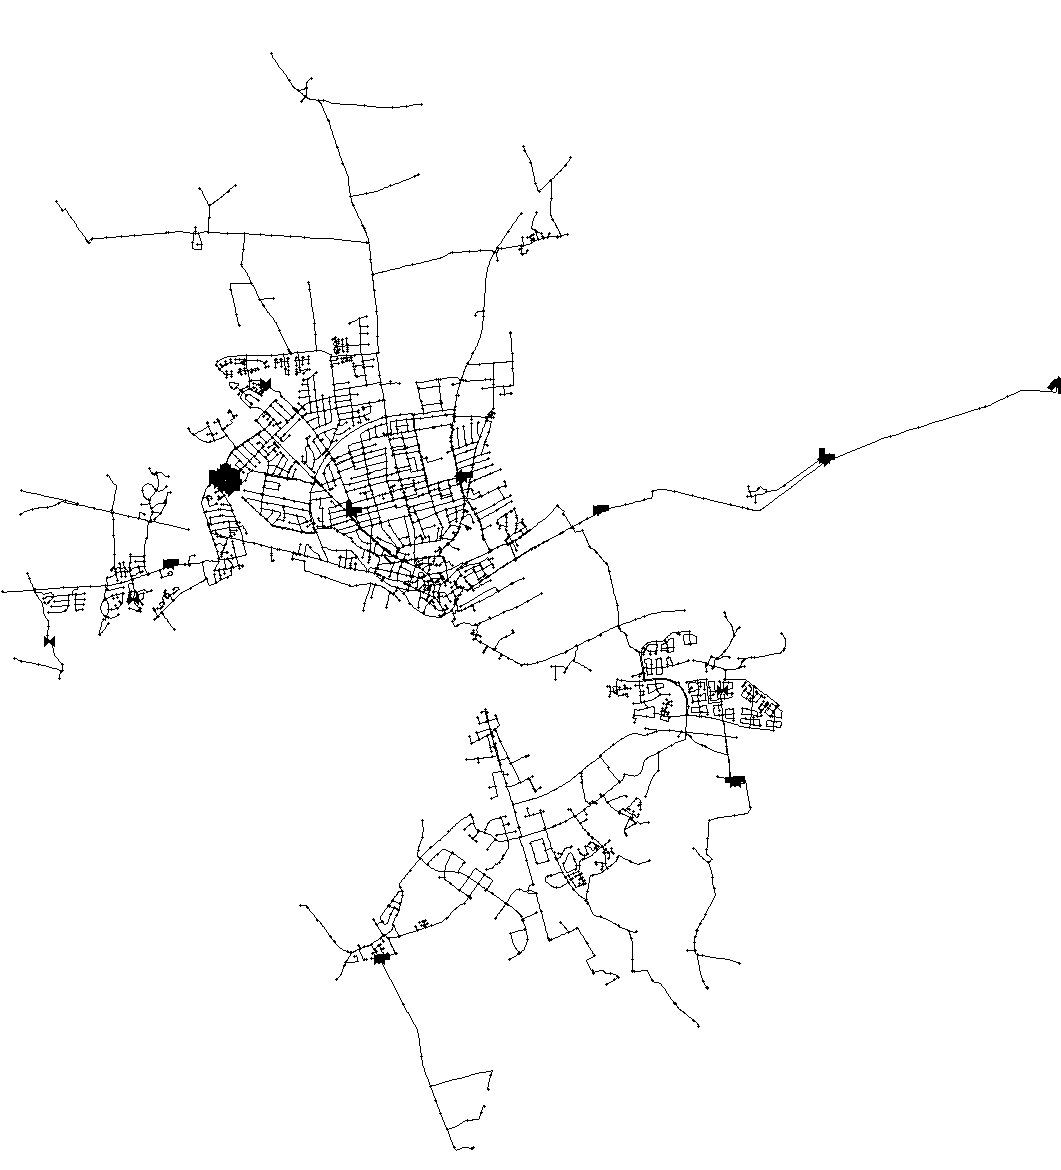
\includegraphics[width=1.5\textwidth]{report/pictures/verdo_pic}};

%     \node[anchor=south west,inner sep=0] at (0,0) {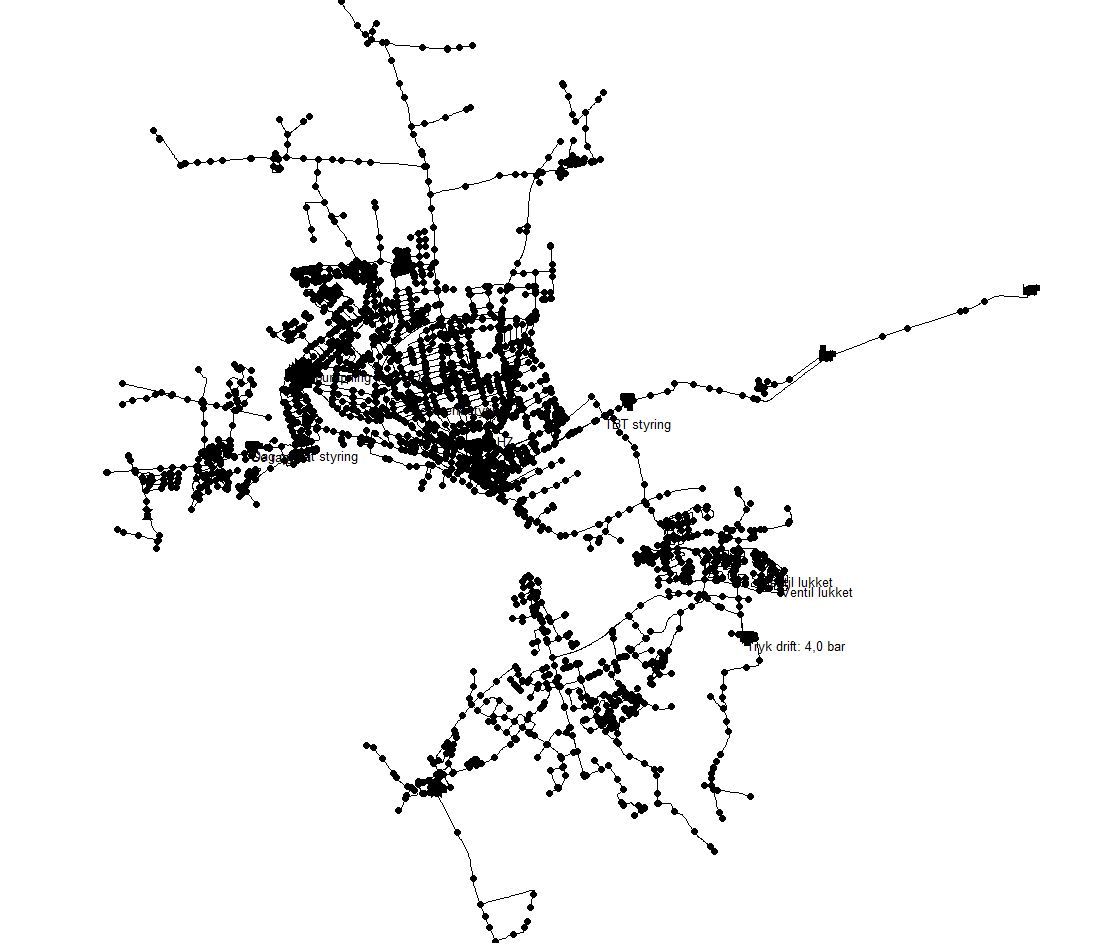
\includegraphics[width=\textwidth]{report/pictures/verdo_pic1}};
            \draw[blue,ultra thick,rounded corners] (3.55,-4.55) rectangle (4.75,-3.7);
             \draw[blue,ultra thick,rounded corners] (5.55,2.15) rectangle (6.8,3);
                      \draw[blue,ultra thick,rounded corners] (-7,2.65) rectangle (-5.75,1.8);
              \draw[blue,line width=0.65mm,rounded corners] (10.05,4.35) rectangle (11.25,3.55);
 \node[black] at (6.05,3.5) {\Large Bunkedal};
   \node[black] at (10.55,4.8) {\Large Østrup Skov};
      \node[black] at (5.6,-4.85) {\Large Vilstrup};
     \node[black] at (-8.55,3) {\Large Oust Mølle};
     
     \draw[red,ultra thick,rounded corners] (-2.1,1.85) rectangle (-0.9,2.7);
      \draw[red,ultra thick,rounded corners] (-8,-0.15) rectangle (-6.8,0.7);
           \draw[red,ultra thick,rounded corners] (1.05,1.15) rectangle (2.25,2);
                \draw[red,ultra thick,rounded corners] (-4.35,1.2) rectangle (-3.15,2.05);
                
                 \node[black] at (2.6,0.65) {\Large Toldbodgade};
                 \node[black] at (0.45,2.85) {\Large Hadsundvej};
                 \node[black] at (-6.45,-0.5) {\Large Hornbæk};
                    \node[black] at (1,5) {\Large Hobrovej};
     
 \draw [-latex](0.1,4.7) -- (-3.25,2.35);
\end{tikzpicture}
 
\caption{Reservoirs in the Randers WSS (encircled in red).}
\label{fig:reservoirs_epanet}
\end{figure}

As can be seen, reservoirs are placed in the outer parts of the city, typically next to the main pumping stations. The locations of the six tanks, or tank stations, in the system is are shown in (figref below)

%illustration of WSS
\begin{figure}[H]
\centering

\includegraphics[width=0.35\textwidth]{report/pictures/missingfigure}
\caption{Illustration of a WSS.}
\label{fig:WSS_example}
\end{figure}